\documentclass[10pt]{article}
\usepackage{icmlko}

\icmlmeta{IP 파운데이션 월드모델}{338}{정찰제}{열 하나의 값이 $-$0.09 로 고정이다 --- 이미 축이 아홉이든 열다섯이든}

\begin{document}

\twocolumn[
\icmlheader

\begin{abstract}
노트 337이 같은 아이돌 25행에 앨범 축 둘(덮음 84\% · 열 넷)을 붙이면
$-$0.05 이고 위키 축 넷(덮음 82\% · 열 여덟)을 붙이면 $+$0.07 인 것을 보고,
남은 설명으로 \textbf{``열의 한계값은 이미 있는 열 수에 달렸다''}를 적었다.
\textbf{쟀다. 틀렸다.}

같은 위약 열(값을 섞어 정보를 0 으로 만든 열)을 두 출발점에 붙였다 ---
살아 있는 축이 \textbf{아홉}인 판과 \textbf{열다섯}인 판.

\begin{center}\small
\begin{tabular}{lrrr}
\hline
출발점 & 짝지은 차 & SD & 음수 \\
\hline
축 아홉 & $-$0.0913 & 0.0647 & \textbf{11/12} \\
축 열다섯 & $-$0.0906 & 0.0571 & \textbf{12/12} \\
\hline
\end{tabular}
\end{center}

\textbf{같다.} 소수 셋째 자리까지 같고 부호가 스물넷 중 스물셋에서 음수다.
\textbf{열 하나의 값은 $-$0.09 로 고정이다.}

\textbf{그리고 기준 한 번으로는 거꾸로 읽혔다} --- 재추출 없이 한 번 재면
축 아홉에서 $-$0.135, 축 열다섯에서 $-$0.022 로 \textbf{여섯 배} 차이로
보인다. 노트 330이 ``오염된 자로 잰 것은 방향까지 뒤집힌다''고 했는데,
여기서는 자가 멀쩡한데 \textbf{한 번만 재서} 뒤집혔다.

\textbf{그래서 값표를 만들 수 있다.} 아이돌(유보 25행)에서

\begin{center}\footnotesize
\begin{tabular}{lrrr}
\hline
무엇 & 값$\sim$라벨 & 짝지은 차 & 부호 \\
\hline
위약 열 하나 & --- & $-$0.09 & 23/24 \\
앨범 축 하나(굿즈) & $+$0.542 & $-$0.046 & 10/12 \\
앨범 축 둘 & --- & $-$0.071 & 11/12 \\
\textbf{위키 축 넷} & --- & \textbf{$+$0.074} & \textbf{11/12} \\
\hline
\end{tabular}
\end{center}

\textbf{열값 $-$0.09 를 넘어야 붙일 값이 있고, 넷 중 하나만 넘었다.}
\end{abstract}
]

\section{두 출발점}

\texttt{lab/idolset.build(scramble=...)} 이 축의 \emph{값만} 섞는다 ---
열 수 · 관측 무늬 · 결측 자리가 그대로고 정보만 없다(값$\sim$라벨
$+$0.542 $\to$ $-$0.009). 그 열을 두 판에 붙였다.

\begin{center}\footnotesize
\begin{tabular}{lrl}
\hline
판 & 살아 있는 축 & 무엇이 있나 \\
\hline
\texttt{idolwide} & 9 & 공유 다섯 $+$ 달력 \\
\texttt{idolwide\_full} & 15 & $+$ 위키 넷 $+$ 검색 넷 \\
\hline
\end{tabular}
\end{center}

\begin{figure*}[t]
\centering
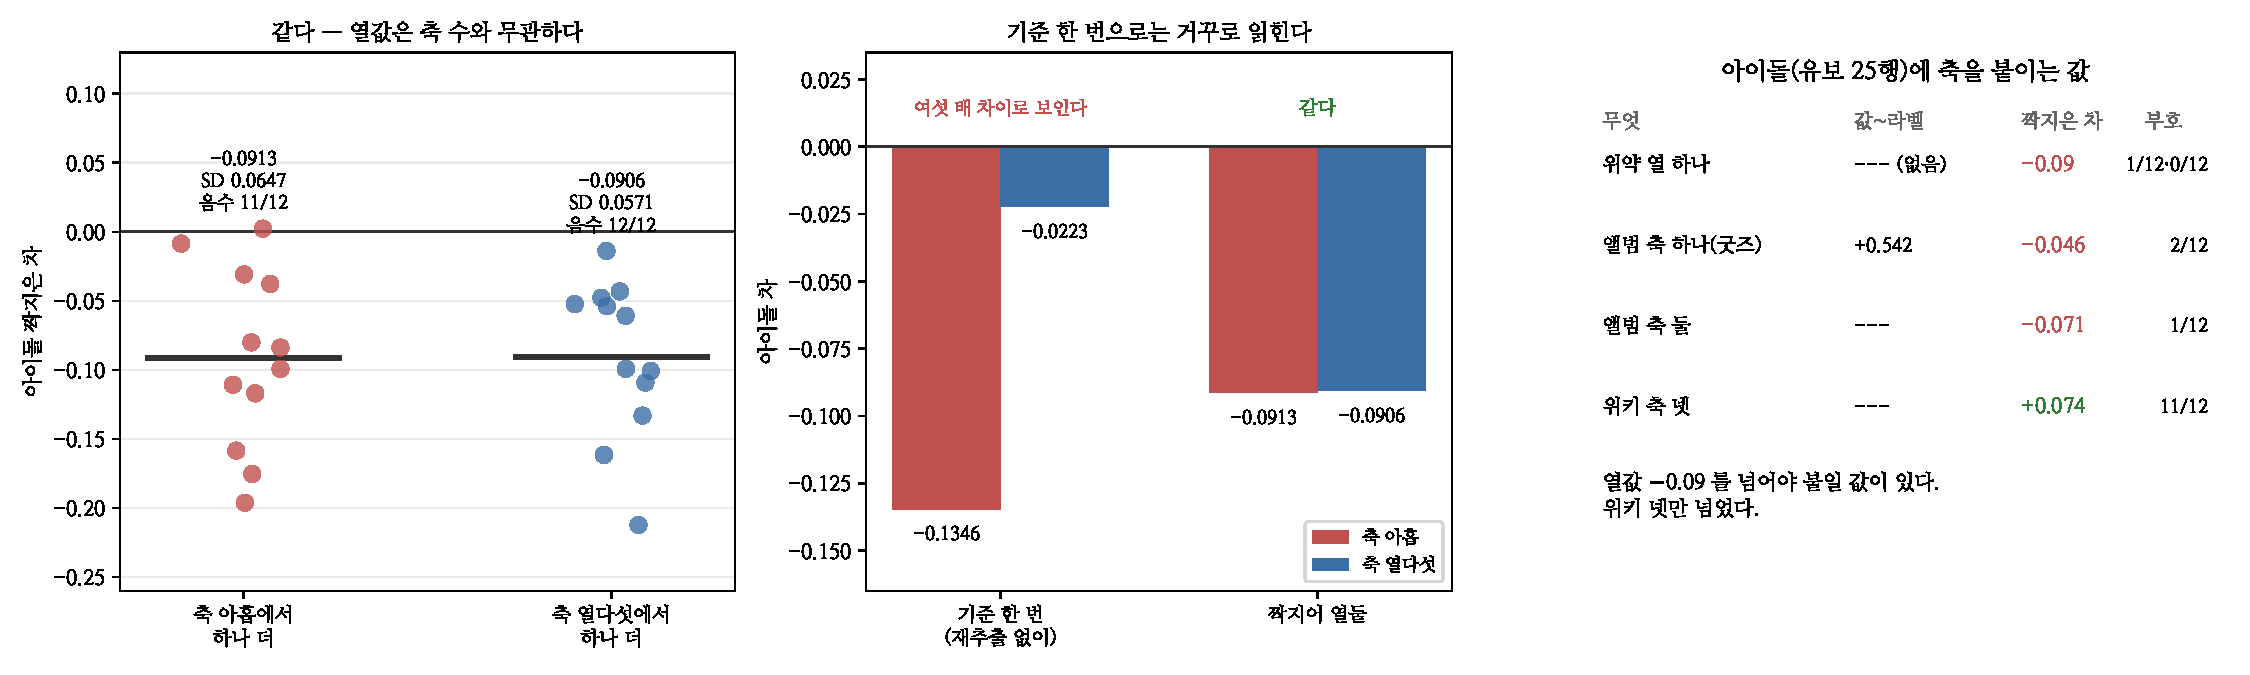
\includegraphics[width=\textwidth]{figs/price.pdf}
\caption{왼쪽 --- 두 출발점의 짝지은 차. 가운데 --- 한 번 재면 거꾸로
읽힌다. 오른쪽 --- 아이돌 값표.}
\end{figure*}

\section{한 번 재면 거꾸로 읽힌다}

\begin{center}\small
\begin{tabular}{lrr}
\hline
 & 축 아홉 & 축 열다섯 \\
\hline
기준 한 번 & $-$0.1346 & $-$0.0223 \\
\textbf{짝지어 열둘} & \textbf{$-$0.0913} & \textbf{$-$0.0906} \\
\hline
\end{tabular}
\end{center}

기준값만 보면 \textbf{여섯 배} 차이다. 짝지어 재면 \textbf{같다.}
노트 331이 아이돌 학습SE 를 0.109 로 쟀으니 한 번의 차는 그 크기로
흔들린다 --- \textbf{$-$0.13 과 $-$0.02 의 차이가 딱 그만큼이다.}

\paragraph{이번에는 미리 안 적었다} 전등록에 이 갈래를 안 넣고 기준값을
먼저 봤다. 그 순간 ``축이 적을수록 위약 열이 비싸다''는 이야기가 곧장
떠올랐다 --- \emph{나무가 쓸 것이 적으면 쓰레기라도 쓴다} 는 그럴듯한
기제까지 같이. \textbf{짝지어 재니 없다.} 노트 133의 규약이 ``첫 양수를
그대로 채택하지 않는다''인데 여기서는 \textbf{첫 \emph{차이}}였다.

\section{값표}

\begin{center}\footnotesize
\begin{tabular}{lrrl}
\hline
아이돌에 붙인 것 & 열 & 짝지은 차 & 부호 \\
\hline
위약 열 하나 & 2 & $-$0.09 & 23/24 \\
앨범 축 하나 & 2 & $-$0.046 & 10/12 \\
앨범 축 둘 & 4 & $-$0.071 & 11/12 \\
\textbf{위키 축 넷} & 8 & \textbf{$+$0.074} & 11/12 \\
\hline
\end{tabular}
\end{center}

\textbf{값이 열 수에 비례하지 않는다} --- 축 하나(열 둘)가 $-$0.046 이고
축 둘(열 넷)이 $-$0.071 로 1.5배뿐이다. \textbf{열이 아니라 ``열을 더한다''는
사건 자체에 값이 붙는다.}

그리고 \textbf{위키 축 넷은 열 여덟인데 $+$0.074 다.} 열값을 물고도
남았다는 뜻이니 \textbf{정보가 최소 $+$0.16 어치}다(위약 넷이 $-$0.09 쯤
든다고 보면).

\section{남은 것}
\begin{center}\footnotesize
\begin{tabular}{ll}
\hline
갈래 & 왜 \\
\hline
\textbf{다른 도메인의 열값} & 유보 711행에서도 $-$0.09 인가 \\
열값이 유보 수를 따르나 & 25 · 104 · 300 · 711 로 재라 \\
표시자 열만 빼면 & 값 열만 실으면 반값인가 \\
\textbf{판 전체 축을 줄이면} & 스물셋 중 안 버는 것 \\
\hline
\end{tabular}
\end{center}

\paragraph{규약} \textbf{차이도 한 번 재면 안 된다.} 이 실험실은 ``첫
양수를 그대로 채택하지 않는다''(노트 133)를 지켜 왔는데 그것은 \emph{크기}
에 대한 규약이었다. 오늘 뒤집힌 것은 \textbf{두 조건 사이의 차이}다 ---
$-$0.135 대 $-$0.022 를 보고 ``축이 적으면 더 비싸다''는 법칙과 그 기제를
한 문장에 만들었고, 짝지어 재니 둘이 같았다. \textbf{그럴듯한 기제가
붙는 순간이 제일 위험하다} --- 그때는 이미 설명이 있으니 다시 재고 싶지
않아진다.

\end{document}
